\chapter{Performance Evaluation}
In this chapter, we will present the performance evaluation of DeAr and demonstrate its capability of efficient and fast arithmetic.
\section{Experiment Setup}
\label{sec:evaluation:setup}
%\\\indent
We prepared two benchmark suites for the experiment.
The first benchmark suite is adapted from the BLAS~\cite{blas} library, 
which contains various matrix arithmetic subprograms that are crucial in wireless communication.
The second benchmark suite include general DSP application kernels selected from classic DSP benchmark suites, BDTI~\cite{btdi} and DSPstone~\cite{dspstone}.
Table~\ref{tab:op} lists the operation profiling of two benchmark suites, 
where each subprogram/kernel comprises three primitive operations, addition, multiplication and shifting.
\begin{table}[!ht]
    \centering
    \caption{Operation profiling of two benchmark suites}
    \label{tab:op}
    \resizebox{\columnwidth}{!}
    {
        \begin{tabular}{|c|c|c|c|c|c|c|c|c|}
            \hline
            \multicolumn{9}{|c|}{\textbf{Basic linear algebra subprograms (BLAS)}} \\ \hline
            Benchmark              & AXPY   & MV     & MM      & INV      & CAXPY  & CMV  & CMM    & CINV  \\ \hline
            \# add            &  32    &  56    &   48    &    75    &  128   & 132  &   90   &  88   \\ \hline
            \# mul            &  32    &  64    &   64    &   172    &  128   & 144  &  108   & 114   \\ \hline
            \# sht            &   0    &   0    &    0    &     0    &    0   &   0  &    0   &   0   \\ \hline
            \# op             &  64    & 120    &  112    &   247    &  256   & 276  &  198   & 202   \\ \hline
            \multicolumn{9}{|c|}{\textbf{General DSP application kernels}}                     \\ \hline
            Benchmark              & FIR    & CFIR   & LPFIR   & Biquad   & IT     & DCT  & IMDCT  & FFT   \\ \hline
            \# add            & 15     &  62    &   15    &    8     &  32    &  29  &   21   &  23   \\ \hline
            \# mul            & 16     &  64    &    8    &    9     &   0    &  12  &   11   &  10   \\ \hline
            \# sht            &  0     &   0    &    0    &    0     &  10    &   9  &    9   &   0   \\ \hline
            \# op             & 31     & 126    &   23    &   17     &  42    &  50  &   41   &  33   \\ \hline
        \end{tabular}
    }
\end{table}
\\\indent Figure~\ref{fig:sim} shows the simulation environment of the experiment.
The design under test (DUT) was replaced in accordance with various DSP architectures to be evaluated, 
which include DeAr, RISC, VLIW and other similar works.
The instruction unit provides stimulus to the DUT based on the IM,
and the L/S unit handles data between the DUT and DM.
We implemented the hardware with UMC 65nm cell library, 
and evaluated area and power with Synopsys Design Compiler and Synopsys Prime Time under certain timing constraints.
\vspace{\textfig}
\begin{figure}[!ht] 
    \centering
    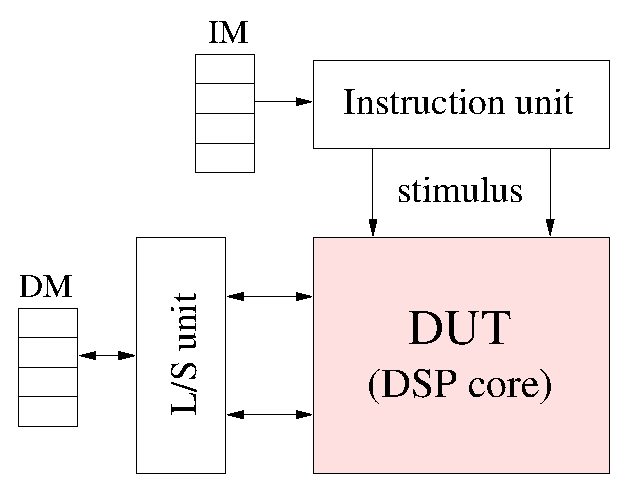
\includegraphics[width=0.6\textwidth]{./figs/sim.eps}
    \caption{Simulation environment}
    \label{fig:sim}
\end{figure}
\\\indent It is important to note that we focused on single-core architectures instead of the multi-core ones in the experiment.
Currently, benchmark results of multi-core systems are highly correlated with the amount of optimization applied to the interconnection and the memory subsystem~\cite{trends}.
Moreover, the programming language also plays a crucial role in multi-core system performance, 
but popular ones such as CUDA, OpenCL and OpenMP are still contending for adoption as the industry standard.
Consequently, the development of a fair benchmark suiting for multi-core DSP platforms is still an open field of study~\cite{landscape}.
Owing to aforementioned issues, we believe benchmarking the single-core DSPs can present more objective evaluation, 
as well as reveal deeper and purer insights into DeAr.
\section{Pre-synthesis Analysis}
{
    \subsection{Operations per Cycle}
    Operations per cycle (OPC) evaluates the utilization rate of the FUs.
    This metric is obtained by statically scheduling operations of a DSP kernel for various architectures.
    Under the performance requirement of target applications, OPC helps to determine the timing constraint for hardware synthesis, 
    where higher OPC brings looser timing constraint, which result in lower cost from the post-synthesis hardware.
    Table~\ref{tab:opc} profiles the OPC of the DSP cores with the assumption that every operation consumes exactly one clock cycle.
    \\\indent The OPC of the scalar processor is fixed to in all benchmarks because of the limitation of the single-issue datapath.
    On the contrary, benefiting from wide issue-width and dedicated ports for each FU, 
    VLIW gains the highest OPC in all benchmarks and thus be considered to be the best case in regard to FUs utilization.
    As an evolved design of VLIW, DeAr gains approximating OPC, with only 1.11\% and 4.26\% loss in two benchmark suites compared with VLIW.
    The slight loss results from the constraint of access pattern in sequential-access banked RF.
    The OPC of composite FU architecture is highly correlated with the cascade order and the benchmark characteristic. 
    On average, the MSA order gains better OPC than the AMS order, 
    but it still under-performed by 12.3\% and 17.7\% in two benchmarks compared with VLIW.
    \begin{table}[!ht]
        \centering
        \caption{Operations per cycle profiling}
        \label{tab:opc}
        \resizebox{\columnwidth}{!}
        {
            \begin{tabular}{|c|c|c|c|c|c|c|c|c|c|}
                \hline
                 \multicolumn{10}{|c|}{\textbf{Basic linear algebra subprograms (BLAS)}} \\ \hline
                Benchmark  &  AXPY  &  MV  &  MM  &  MINV  &  CAXPY  &  CMV  &  CMM  &  CMINV  &  Average \\ \hline 
                VLIW  &   1.94  &   1.85  &   1.72  &   1.44  &   1.97  &   1.89  &   1.80  &   1.76  &   1.79     \\ \hline 
                DeAr  &   1.94  &   1.85  &   1.72  &   1.40  &   1.97  &   1.89  &   1.80  &   1.62  &   1.77     \\ \hline
                Composite-MSA  &   2.00  &   1.88  &   1.75  &   1.37  &   1.33  &   1.35  &   1.38  &   1.53  &   1.57     \\ \hline 
                Composite-AMS  &   1.00  &   1.00  &   1.00  &   1.02  &   1.00  &   1.00  &   1.00  &   1.04  &   1.01     \\ \hline 
                Scalar  & 1.0  & 1.0  & 1.0  & 1.0  & 1.0  & 1.0  & 1.0  & 1.0  & 1.0 \\ \hline 
                \multicolumn{10}{|c|}{\textbf{General DSP application kernels}}                     \\ \hline
                Benchmark  &  FIR  &  CFIR  &  LPFIR  &  Biquad  &  IT  &  DCT  &  IMDCT  &  FFT  &  Average \\ \hline 
                VLIW  &   1.82  &   1.91  &   1.67  &   1.54  &   1.33  &   1.61  &   1.86  &   1.38  &   1.64     \\ \hline 
                %         ^fix 1.67 to 1.82              ^fix 1.42 to 1.54                                 ^ fix 1.61 to 1.62
                DeAr  &   1.82  &   1.91  &   1.67  &   1.54  &   1.33  &   1.47  &   1.46  &   1.32  &   1.57     \\ \hline 
                Composite-MSA  &   1.94  &   1.34  &   1.44  &   1.42  &   1.31  &   1.14  &   1.28  &   1.06  &   1.35     \\ \hline 
                Composite-AMS  &   1.00  &   1.00  &   1.53  &   1.21  &   1.14  &   1.61  &   1.52  &   1.27  &   1.29     \\ \hline 
                Scalar  & 1.0  & 1.0  & 1.0  & 1.0  & 1.0  & 1.0  & 1.0  & 1.0  & 1.0 \\ \hline 
            \end{tabular}
        }
    \end{table}
    \subsection{Register file access rate}
    Register file access rate provides a quantitative measurement of the register file activity, 
    which makes up the majority of power consumption in DSP cores.
    It is calculated dividing the real number of register file accesses by the worst case number of accesses.
    Table~\ref{tab:rpd} profiles the RF access rate of each architecture in regard to various benchmarks.
    Under the assumption of single cycle datapaths, conventional architectures, scalar and VLIW, 
    lack bypassing capability and write back arithmetic results every cycle, 
    We referred to such a scenario as the worst case in regard to RF access, 
    and thus their RF access rate is fixed to 1.0.
    On the contrary, DeAr leverages its accumulators and novel scheduling mechanism to explore data bypassing opportunities. 
    As a result, its RF access rate was reduced to 0.69 and 0.73, 
    and out-performed the best composite order, MSA, which had the RF access rate of 0.77 and 0.82 respectively in two benchmark suites.
    \begin{table}[!ht]
        \centering
        \caption{Register file access rate profiling}
        \label{tab:rpd}
        \resizebox{\columnwidth}{!}
        {
            \begin{tabular}{|c|c|c|c|c|c|c|c|c|c|}
                \hline
                 \multicolumn{10}{|c|}{\textbf{Basic linear algebra subprograms (BLAS)}} \\ \hline
                Benchmark  &  AXPY  &  MV  &  MM  &  MINV  &  CAXPY  &  CMV  &  CMM  &  CMINV  &  Average \\ \hline 
                DeAr  &   0.67  &   0.69  &   0.71  &   0.67  &   0.67  &   0.68  &   0.70  &   0.71  &   0.69     \\ \hline
                Composite-MSA  &   0.67  &   0.69  &  0.71  &   0.82  &   0.83  &   0.83  &   0.82  &   0.77  &  0.77     \\ \hline 
                Composite-AMS  &   1.0  &   1.00  &   1.00  &   0.98  &   1.00  &   1.00  &   1.00  &   0.97  &   0.99     \\ \hline 
                VLIW  &   1.00  &   1.00  &   1.00  &   1.00  &   1.00  &   1.00  &   1.00  &   1.00  &   1.00     \\ \hline 
                Saclar  &   1.00  &   1.00  &   1.00  &   1.00  &   1.00  &   1.00  &   1.00  &   1.00  &   1.00     \\ \hline 
                \multicolumn{10}{|c|}{\textbf{General DSP application kernels}}                     \\ \hline
                Benchmark  &  FIR  &  CFIR  &  LPFIR  &  Biquad  &  IT  &  DCT  &  IMDCT  &  FFT  &  Average \\ \hline 
                DeAr  &   0.68  &   0.67  &  0.60  &   0.57  &   0.85  &   0.74  &   0.86  &   0.82  &   0.73     \\ \hline 
                Composite-MSA  &   0.68  &   0.83  &   0.80  &   0.80  &   0.83  &   0.87  &   0.80  &   0.92  &   0.82     \\ \hline 
                Composite-AMS  &   1.00  &   1.00  &   0.77  &   0.88  &   1.00  &   0.76  &   0.84  &   0.86  &   0.87     \\ \hline 
                VLIW  &   1.00  &   1.00  &   1.00  &   1.00  &   1.00  &   1.00  &   1.00  &   1.00  &   1.00     \\ \hline 
                Saclar  &   1.00  &   1.00  &   1.00  &   1.00  &   1.00  &   1.00  &   1.00  &   1.00  &   1.00     \\ \hline 
            \end{tabular}
        }
    \end{table}
    \subsection{Code density}
    To evaluate code density, we defined a new metric, operation per byte (OPB).
    It is calculated by dividing OPC by the instruction issue width in bytes.
    We assumed that the total number of registers in the RF is 32, 
    which implies 5 bits are needed to address the centralized RF, 
    and that each ISA supports less than 8 instructions,
    which implies 3 bits are needed to select the function of an instruction.
    In addition, we took overall average OPC of two benchmark suites from Table~\ref{tab:opc}.

}
\section{Synthesis Result}
{
    \subsection{Area Analysis}
    \vspace{\textfig}
    \begin{figure}[!ht]
        \begin{center}
            \subfigure[BLAS benchmark suite]
            {
                \label{chart:area:blas}
                \includegraphics[width=0.48\textwidth]{charts/area_blas.eps}
            }
            \subfigure[General benchamrk suite]
            {
                \label{chart:area:general}
                \includegraphics[width=0.48\textwidth]{charts/area_general.eps}
            }
        \end{center}
        \caption{Area analysis for DSP cores}
        \label{chart:area}
    \end{figure}

    \subsection{Total Power Consumption Analysis}
    \vspace{\textfig}
    \begin{figure}[!ht]
        \begin{center}
            \subfigure[BLAS benchmark suite]
            {
                \label{chart:power:blas}
                \includegraphics[width=0.48\textwidth]{charts/power_blas.eps}
            }
            \subfigure[General benchamrk suite]
            {
                \label{chart:power:general}
                \includegraphics[width=0.48\textwidth]{charts/power_general.eps}
            }
        \end{center}
        \caption{Total power analysis for DSP cores}
        \label{chart:area}
    \end{figure}

    \subsection{Leakage Power Consumption Analysis}
    \vspace{\textfig}
    \begin{figure}[!ht]
        \begin{center}
            \subfigure[BLAS benchmark suite]
            {
                \label{chart:leakage:blas}
                \includegraphics[width=0.48\textwidth]{charts/leakage_blas.eps}
            }
            \subfigure[General benchamrk suite]
            {
                \label{chart:leakage:general}
                \includegraphics[width=0.48\textwidth]{charts/leakage_general.eps}
            }
        \end{center}
        \caption{Leakage power analysis for DSP cores}
        \label{chart:leakage}
    \end{figure}
}


